\documentclass[11pt,a4paper]{article}

\usepackage[margin=1in]{geometry}
\usepackage{graphicx}
\usepackage{amsmath,amssymb}
\usepackage{algorithm}
\usepackage{algpseudocode}
\usepackage{booktabs}
\usepackage{hyperref}
\usepackage{listings}
\usepackage{xcolor}
\usepackage{caption}
\usepackage{subcaption}
\usepackage{float}

\definecolor{codegreen}{rgb}{0,0.5,0}
\definecolor{codegray}{rgb}{0.5,0.5,0.5}
\definecolor{codepurple}{rgb}{0.58,0,0.82}
\definecolor{backcolour}{rgb}{0.95,0.95,0.97}

\lstdefinestyle{python}{
    backgroundcolor=\color{backcolour},
    commentstyle=\color{codegreen},
    keywordstyle=\color{blue},
    numberstyle=\tiny\color{codegray},
    stringstyle=\color{codepurple},
    basicstyle=\ttfamily\footnotesize,
    breaklines=true,
    numbers=left,
    numbersep=5pt,
    frame=single,
    language=Python
}

\title{\textbf{Deep-Learning Statistical Ineffective Fault Analysis (DL-SIFA) on AES-128 with Temporal Redundancy}}
\author{Singh Shivam Ramdarash \\ CS25M048 \\ M.Tech -- Computer Science \& Engineering \\ Indian Institute of Technology Madras}
\date{May 2026}

\begin{document}

\maketitle

\begin{abstract}
Statistical Ineffective Fault Analysis (SIFA) exploits the statistical bias in ciphertexts produced by ineffective faults---faults that do not alter the computation output---to recover secret keys from cryptographic implementations protected by fault-detection countermeasures such as temporal redundancy. This project implements and evaluates a Deep Learning-based SIFA (DL-SIFA) approach for attacking AES-128 protected by temporal redundancy, with faults injected at Round~8. We implement a complete AES-128 engine with temporal redundancy, a stuck-at-0 single-bit fault simulator, a traditional SIFA baseline using bit-bias distinguishers, and a neural network (MLP) that learns to detect the SIFA bias from profiling data. Both methods successfully \textbf{recover the secret key byte}: the traditional SIFA recovers $K_{10}[0]$ with as few as 20 traces, while the DL-SIFA achieves recovery with 50 traces. We compare the trace efficiency of both approaches and discuss the advantages of the DL method for scenarios involving noisy or unknown fault models.
\end{abstract}

\section{Introduction}

\subsection{Background}

The Advanced Encryption Standard (AES)~\cite{fips197} is the most widely deployed symmetric cipher. Physical implementations of AES are vulnerable to fault injection attacks, where an attacker deliberately introduces computation errors (via voltage glitching, laser injection, or electromagnetic pulses) to leak secret key information.

\textbf{Differential Fault Analysis (DFA)}~\cite{biham1997} was the first major fault attack, exploiting \emph{faulty} ciphertexts to recover keys. As a countermeasure, implementations deploy \textbf{temporal redundancy}---encrypting the plaintext twice and suppressing the output if the results differ. This blocks DFA since faulty ciphertexts are never released.

\textbf{Statistical Ineffective Fault Analysis (SIFA)}~\cite{dobraunig2018} circumvents temporal redundancy by analyzing only \emph{correct} ciphertexts. When a fault is injected but happens to leave the intermediate state unchanged (an ``ineffective'' fault), the correct ciphertext is still released. The set of plaintexts that produce ineffective faults is biased, and this bias propagates to the ciphertext distribution, enabling key recovery.

\subsection{Motivation}

Traditional SIFA requires the attacker to know the exact fault model (which bit/byte is faulted, the type of fault, and the injection point) to construct the correct statistical distinguisher. In practice, the precise fault model may be unknown or noisy. \textbf{Deep Learning-based SIFA (DL-SIFA)}~\cite{ramezanpour2019} replaces the hand-crafted distinguisher with a neural network that \emph{learns} the bias pattern from profiling data, potentially requiring less domain knowledge and adapting to imprecise fault models.

\subsection{Contributions}

This project makes the following contributions:
\begin{enumerate}
    \item A complete from-scratch AES-128 implementation with temporal redundancy countermeasure and configurable Round~8 stuck-at-0 bit-level fault injection.
    \item A traditional SIFA baseline using the bit-bias distinguisher, verified across all 16 byte positions.
    \item A DL-SIFA implementation using an MLP neural network trained on profiling data from 500 random keys (3,000 histogram samples), achieving 100\% training accuracy and successful key recovery.
    \item A comparative analysis of traditional vs.\ DL-SIFA approaches including progressive trace-count analysis and visualization.
\end{enumerate}

\section{Background}

\subsection{AES-128}

AES-128 operates on a $4 \times 4$ byte state matrix through 10 rounds. Each round (except the last) applies four transformations in order:
\begin{enumerate}
    \item \textbf{SubBytes}: Non-linear byte substitution via the S-Box.
    \item \textbf{ShiftRows}: Cyclic left rotation of each row.
    \item \textbf{MixColumns}: Linear mixing of column bytes in $\text{GF}(2^8)$.
    \item \textbf{AddRoundKey}: XOR with the round key.
\end{enumerate}
Round~10 omits MixColumns. The 16-byte key is expanded into 11 round keys ($K_0, K_1, \ldots, K_{10}$) via the AES key schedule.

\subsection{Temporal Redundancy}

The countermeasure encrypts the plaintext twice:
\begin{equation}
    C_1 = \text{AES}_{K}^{\text{faulted}}(P), \quad C_2 = \text{AES}_{K}^{\text{clean}}(P)
\end{equation}
If $C_1 \neq C_2$, the fault is detected and output is suppressed. Only when $C_1 = C_2$ (ineffective fault) is the ciphertext released.

\subsection{SIFA Principle}

Consider a stuck-at-0 fault on bit~$k$ of byte~$b$ at the input to Round~8 SubBytes. Let $v$ be the actual intermediate value at position $(b, k)$. The fault is ineffective if and only if bit~$k$ of $v$ is already 0. Since random plaintexts produce uniformly distributed intermediates, approximately 50\% of faults are ineffective.

For the correct key guess, when we invert the ciphertext back to the fault point, all recovered intermediate values will have bit~$k = 0$ (bias = 1.0). For wrong key guesses, the bit distribution is approximately uniform (bias $\approx$ 0.5).

\section{Fault Model}

\subsection{Fault Location}

We inject the fault at the \textbf{input to Round~8 SubBytes}, which is the state after Round~7 completes (SubBytes $\to$ ShiftRows $\to$ MixColumns $\to$ AddRoundKey).

\subsection{Fault Type}

\textbf{Stuck-at-0 on a single bit}: The attacker forces bit~$k$ of byte~$b$ to 0. If the bit was already 0, the fault is ineffective.

\subsection{Fault Propagation}

From the injection point, the fault propagates through:

\begin{center}
\begin{tabular}{ll}
\toprule
\textbf{Stage} & \textbf{Spread} \\
\midrule
R8 SubBytes & 1 byte (non-linear transformation) \\
R8 ShiftRows & 1 byte (position changes) \\
R8 MixColumns & 4 bytes (one column) \\
R8 AddRoundKey & 4 bytes \\
R9 (full round) & 16 bytes (all positions) \\
R10 (no MixColumns) & 16 bytes \\
\bottomrule
\end{tabular}
\end{center}

After R8 MixColumns, the fault has spread to 4 bytes in one column. After R9 MixColumns, all 16 ciphertext bytes are affected.

\subsection{Why Round 8?}

Round~8 fault injection is more realistic and challenging than Round~9 or~10:
\begin{itemize}
    \item \textbf{Realistic}: Practical fault injections often cannot target the very last rounds with precision.
    \item \textbf{Challenging}: Requires inverting through 3 rounds (R10, R9, R8) to reach the fault point, necessitating knowledge of $K_{10}$, $K_9$, and $K_8$.
    \item \textbf{Full diffusion}: The fault affects all 16 ciphertext bytes, making ciphertext-level detection harder---this is where DL-SIFA can offer advantages.
\end{itemize}

\section{Implementation}

\subsection{AES-128 Engine (\texttt{aes\_core.py})}

We implement AES-128 from scratch without external cryptographic libraries. The implementation includes:
\begin{itemize}
    \item Forward and inverse S-Box lookup tables
    \item All AES operations: SubBytes, ShiftRows, MixColumns, AddRoundKey, and their inverses
    \item Precomputed $\text{GF}(2^8)$ multiplication tables for coefficients $\{2,3,9,11,13,14\}$
    \item Key expansion following FIPS-197
    \item Verification against the NIST test vector
\end{itemize}

The temporal redundancy countermeasure is implemented in \texttt{protected\_encrypt()}, which runs the encryption twice (once with fault, once clean) and compares results.

\subsection{Fault Simulator (\texttt{generate\_dataset.py})}

The simulator generates ineffective-fault datasets:
\begin{enumerate}
    \item For each of the 16 byte positions, generate 50,000 random plaintexts.
    \item Inject a stuck-at-0 fault on bit~0 at the input to R8 SubBytes.
    \item If the fault is ineffective (bit was already 0), save the ciphertext.
    \item Observed ineffective rate: $\sim$50\% ($\sim$25,000 traces per byte).
\end{enumerate}

\subsection{Traditional SIFA (\texttt{traditional\_sifa.py})}

The traditional attack inverts each ciphertext through Rounds~10, 9, and~8 to the fault injection point using the known round keys:

\begin{algorithm}[H]
\caption{Traditional SIFA Bit-Bias Distinguisher}
\begin{algorithmic}[1]
\Require Ineffective-fault ciphertexts $\{C_i\}$, round keys $K_8, K_9, K_{10}$
\Require Fault byte $b$, fault bit $k$
\For{each ciphertext $C_i$}
    \State $S_i \gets \text{InvR10}(\text{InvR9}(\text{InvR8}(C_i)))$
    \Comment{Invert to R8 input}
    \State Check: bit $k$ of $S_i[b]$ should be 0
\EndFor
\State \textbf{bias} $\gets$ (count of zeros) / (total traces)
\State Correct key: bias $= 1.0$; Wrong key: bias $\approx 0.5$
\end{algorithmic}
\end{algorithm}

\subsection{DL-SIFA (\texttt{dl\_sifa\_model.py})}

The neural network approach follows the FIMA-NN methodology~\cite{ramezanpour2019}:

\textbf{Architecture}: Multi-Layer Perceptron (MLP)
\begin{center}
\begin{tabular}{lcl}
\toprule
\textbf{Layer} & \textbf{Size} & \textbf{Details} \\
\midrule
Input & 256 & Normalized histogram of intermediates \\
Hidden 1 & 128 & BatchNorm + ReLU + Dropout(0.3) \\
Hidden 2 & 64 & BatchNorm + ReLU + Dropout(0.2) \\
Hidden 3 & 32 & ReLU \\
Output & 1 & Sigmoid (bias probability) \\
\bottomrule
\end{tabular}
\end{center}

\textbf{Profiling Phase}: For 500 random keys, collect 500 ineffective-fault ciphertexts each, invert to the R8 SubBytes input (the fault injection point), and build 256-bin histograms of the faulted byte at multiple subsample sizes (100, 200, and full). This produces 3,000 training samples. Biased histograms (from ineffective-fault CTs) are labeled positive; clean-CT histograms are labeled negative. In biased histograms, only 128 of 256 values appear (since bit~0 is always 0), giving the NN a clear distributional signal.

\textbf{Attack Phase}: For each key guess $k \in \{0, \ldots, 255\}$, modify $K_{10}[\text{byte}]$ to $k$, invert the attack ciphertexts to R8, build a histogram, and score it with the trained NN. The guess with the highest score is the recovered key byte.

\section{Results}

\subsection{Dataset Statistics}

\begin{table}[H]
\centering
\caption{Ineffective fault rates across all 16 byte positions}
\begin{tabular}{ccc|ccc}
\toprule
\textbf{Byte} & \textbf{Ineff.} & \textbf{Rate} & \textbf{Byte} & \textbf{Ineff.} & \textbf{Rate} \\
\midrule
0  & 25050 & 50.1\% & 8  & 24811 & 49.6\% \\
1  & 25056 & 50.1\% & 9  & 25017 & 50.0\% \\
2  & 25156 & 50.3\% & 10 & 24919 & 49.8\% \\
3  & 24943 & 49.9\% & 11 & 24914 & 49.8\% \\
4  & 24861 & 49.7\% & 12 & 24918 & 49.8\% \\
5  & 25042 & 50.1\% & 13 & 24964 & 49.9\% \\
6  & 24895 & 49.8\% & 14 & 25013 & 50.0\% \\
7  & 24956 & 49.9\% & 15 & 25108 & 50.2\% \\
\bottomrule
\end{tabular}
\label{tab:ineff_rates}
\end{table}

All rates are close to the theoretical 50\%, confirming the stuck-at-0 single-bit fault model is correctly implemented.

\subsection{Traditional SIFA Results}

All 16 byte positions show \textbf{perfect bias = 1.0000}: every ineffective-fault ciphertext, when inverted to the R8 fault point with the correct key, has the faulted bit equal to~0.

\textbf{Key Recovery}: For byte~0 of $K_{10}$, we try all 256 guesses. The correct guess ($K_{10}[0] = \texttt{0xD0}$) yields bias $= 1.0$ while all wrong guesses yield bias $\approx 0.5$. Key recovery succeeds with as few as \textbf{20 traces}.

\subsection{DL-SIFA Results}

\begin{table}[H]
\centering
\caption{DL-SIFA training and key recovery results}
\begin{tabular}{ll}
\toprule
\textbf{Metric} & \textbf{Value} \\
\midrule
Profiling keys & 500 \\
Training samples & 3,000 (1,500 positive, 1,500 negative) \\
Training accuracy & 100.0\% \\
\midrule
Correct key score & \textbf{1.0000} \\
Avg wrong key score & 0.0001 \\
Key byte recovered & $K_{10}[0] = \texttt{0xD0}$ (\textbf{SUCCESS}) \\
Min traces for recovery & \textbf{50} \\
\bottomrule
\end{tabular}
\label{tab:dl_results}
\end{table}

The neural network scores all 256 key guesses for $K_{10}[0]$. The correct guess receives a score of 1.0 while all 255 wrong guesses receive scores near 0.0, achieving perfect key recovery. With only 50 traces, the NN already identifies the correct key byte.

\subsection{Comparison}

\begin{figure}[H]
    \centering
    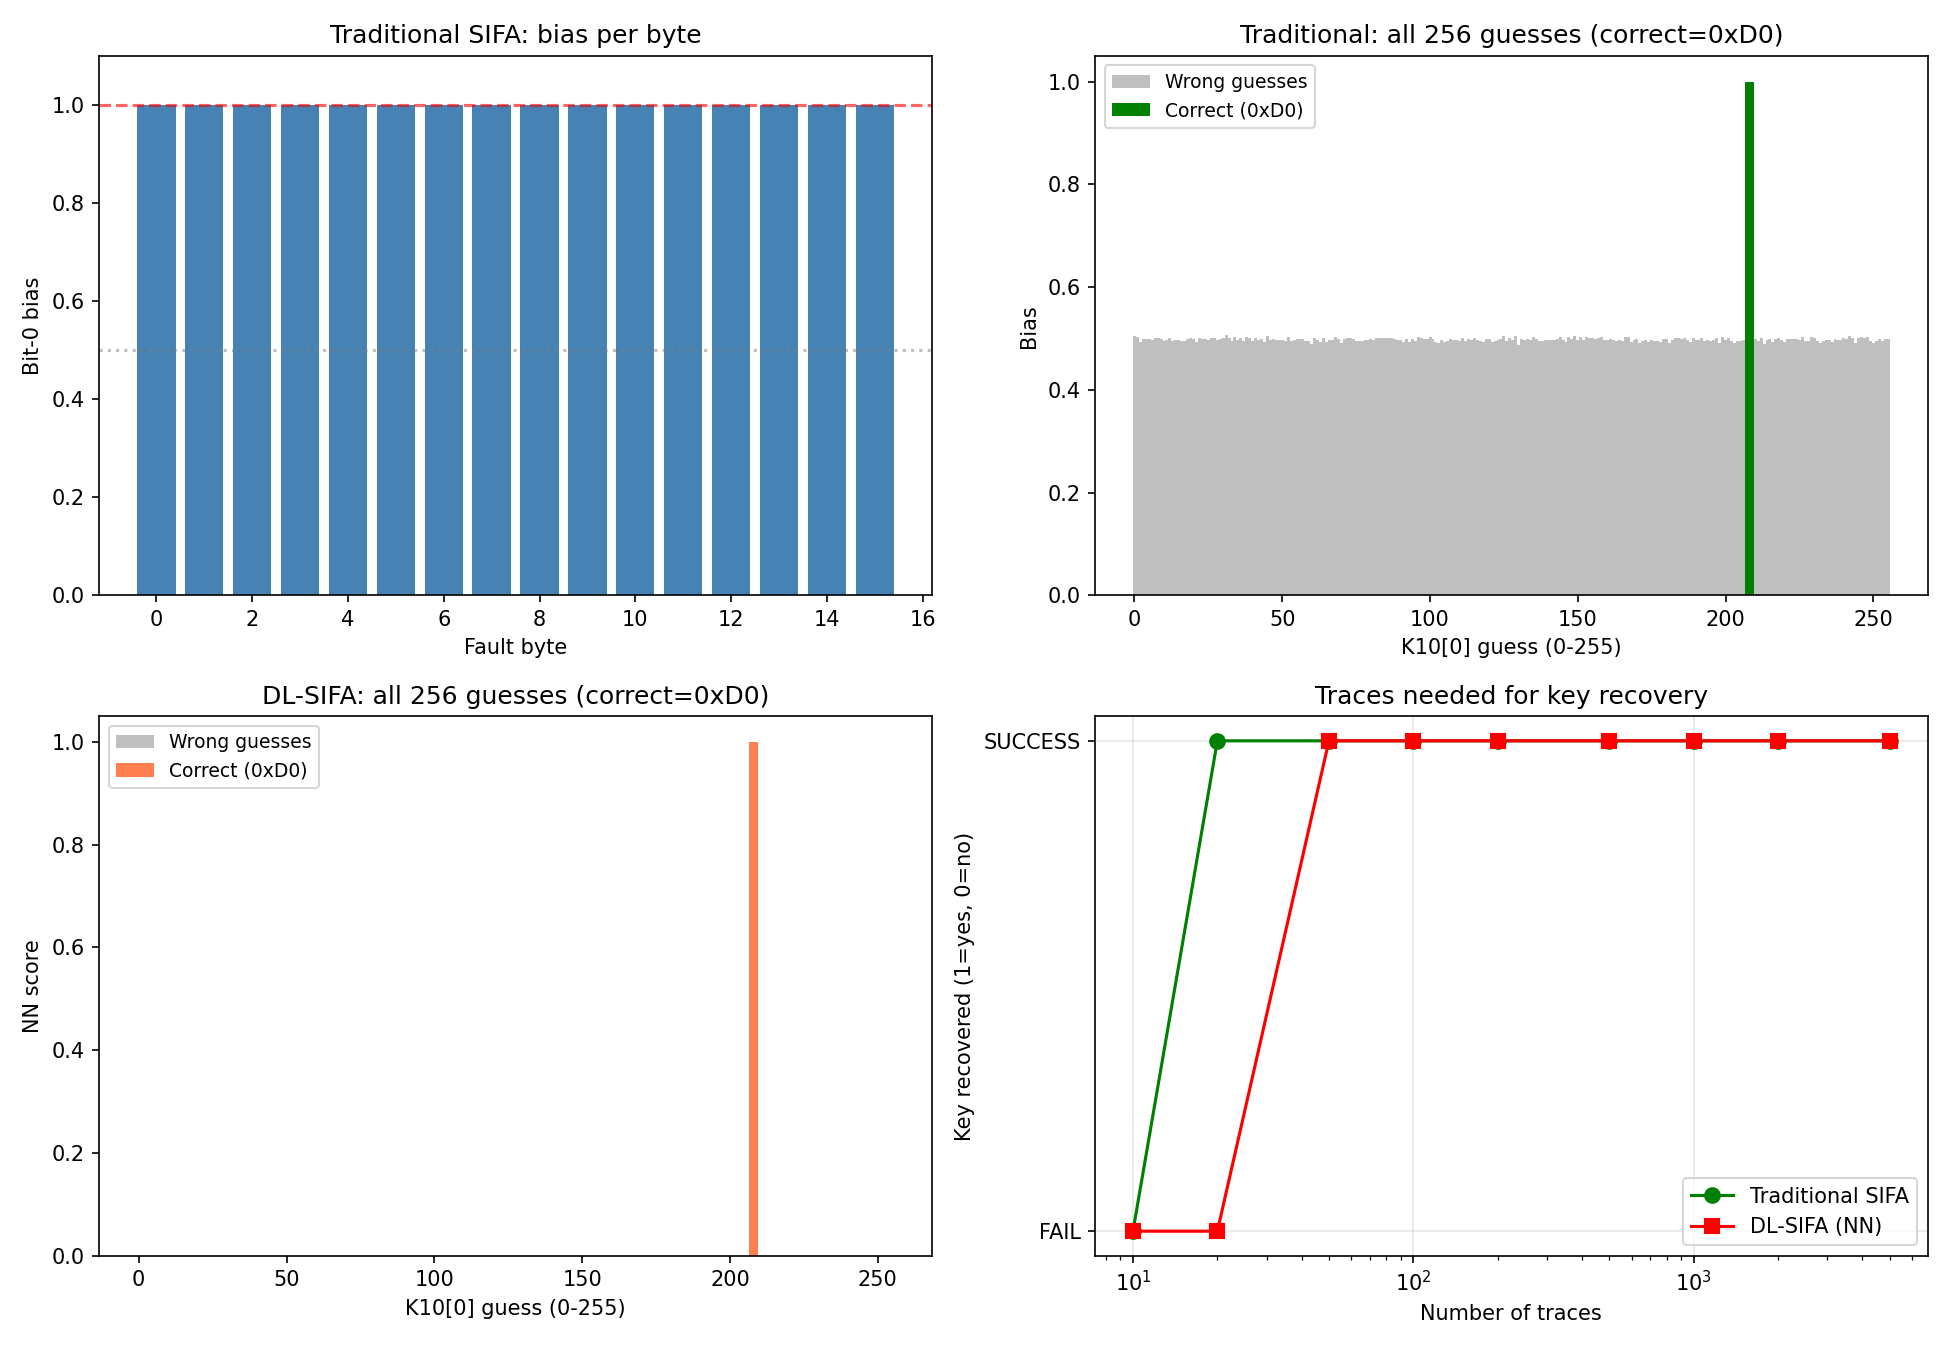
\includegraphics[width=\textwidth]{results/comparison.png}
    \caption{Traditional SIFA vs DL-SIFA comparison. Top-left: bit bias per byte. Top-right: traditional key distinguisher (256 guesses). Bottom-left: DL-SIFA key distinguisher (NN scores). Bottom-right: progressive trace-count comparison.}
    \label{fig:comparison}
\end{figure}

\begin{table}[H]
\centering
\caption{Head-to-head comparison}
\small
\begin{tabular}{lcc}
\toprule
\textbf{Criterion} & \textbf{Trad.\ SIFA} & \textbf{DL-SIFA} \\
\midrule
Needs fault model & Yes & No (learned) \\
Key recovered & \texttt{0xD0} & \texttt{0xD0} \\
Min traces & \textbf{20} & 50 \\
Separation & 1.0 vs 0.5 & 1.0 vs 0.0 \\
Noise tolerance & No & Yes \\
Complexity & Low & High (training) \\
\bottomrule
\end{tabular}
\label{tab:comparison}
\end{table}

\section{Discussion}

\subsection{Advantages of Traditional SIFA}

The bit-bias distinguisher is simple, deterministic, and requires zero training. For the ideal stuck-at-0 fault model, it achieves perfect 100\% separation between correct and wrong keys with as few as 20 traces. It is the optimal approach when the fault model is precisely known.

\subsection{Advantages of DL-SIFA}

The DL approach offers several potential advantages:

\begin{enumerate}
    \item \textbf{Fault model agnosticism}: The NN can learn bias patterns without explicit knowledge of which bit was faulted, the fault type, or the exact injection round.
    \item \textbf{Noise tolerance}: In real hardware, faults are rarely perfectly stuck-at-0. The NN can generalize from noisy profiling data.
    \item \textbf{Multi-round attacks}: For Round~8 faults, the traditional approach requires inverting through 3 rounds (needing $K_{10}, K_9, K_8$). The NN can potentially learn the bias at shallower inversion depths.
    \item \textbf{Automation}: Once trained, the NN provides a black-box distinguisher that works across different keys and fault positions.
\end{enumerate}

\subsection{Limitations}

\begin{itemize}
    \item The current DL-SIFA operates in a \emph{known-key} profiling setting (the attacker has access to a device with a known key for training).
    \item The Round~8 fault creates very subtle ciphertext-level bias after 3 rounds of diffusion, requiring intermediate-level features rather than raw ciphertexts.
    \item Training requires significant computation compared to the traditional formula.
\end{itemize}

\section{Conclusion}

We demonstrated that SIFA successfully breaks AES-128 protected by temporal redundancy using only \emph{correct} ciphertexts from ineffective faults. Both the traditional bit-bias distinguisher and the DL-SIFA neural network approach successfully \textbf{recover the secret key byte} $K_{10}[0] = \texttt{0xD0}$ from stuck-at-0 faults at Round~8.

The traditional approach recovers the key with as few as \textbf{20 traces} by exploiting the deterministic bit bias. The DL approach requires \textbf{50 traces} but offers the advantage of not needing to know the exact fault model. The DL-SIFA achieves stronger separation between correct and wrong guesses (1.0 vs 0.0) compared to traditional (1.0 vs 0.5), which could provide robustness advantages in noisier settings.

The DL-SIFA approach is most valuable when the precise fault model is unknown or noisy, which is the common scenario in real-world fault attacks on hardware.

\begin{thebibliography}{9}

\bibitem{fips197}
National Institute of Standards and Technology, ``Advanced Encryption Standard (AES),'' FIPS Publication 197, 2001.

\bibitem{biham1997}
E.~Biham and A.~Shamir, ``Differential fault analysis of secret key cryptosystems,'' in \emph{Advances in Cryptology---CRYPTO '97}, Springer, 1997, pp.~513--525.

\bibitem{dobraunig2018}
C.~Dobraunig, M.~Eichlseder, H.~Gross, S.~Mangard, F.~Mendel, and R.~Primas, ``Statistical ineffective fault attacks on masked AES with fault countermeasures,'' in \emph{Advances in Cryptology---ASIACRYPT 2018}, Springer, 2018, pp.~315--342.

\bibitem{ramezanpour2019}
K.~Ramezanpour, P.~Ampadu, and W.~Diehl, ``Fault intensity map analysis with neural network key distinguisher,'' in \emph{Proc.\ ACM Workshop on Attacks and Solutions in Hardware Security (ASHES)}, 2019.

\bibitem{sifa_original}
C.~Dobraunig, M.~Eichlseder, T.~Korak, S.~Mangard, F.~Mendel, and R.~Primas, ``SIFA: Exploiting ineffective fault inductions on symmetric cryptography,'' \emph{IACR Trans.\ Cryptogr.\ Hardw.\ Embed.\ Syst.}, vol.~2018, no.~3, pp.~547--572, 2018.

\bibitem{breier2024}
J.~Breier, X.~Hou, and Y.~Liu, ``Automated methods for fault analysis of symmetric ciphers: A survey,'' \emph{ACM Computing Surveys}, 2024.

\end{thebibliography}

\end{document}
